\chapter{Integrated Exploration Methodology for Data Interleaving and Data-to-Memory Mapping on SIMD architectures}

\begin{center}
Iason Filippopoulos, Namita Sharma, Francky Catthoor, \\ Per Gunnar Kjeldsberg and Preeti Ranjan Panda
\\
ACM Transactions on Embedded Computing Systems
\\
Submitted in 2015
\end{center}
\afterpage{\null\newpage}
\newpage

\vspace*{\fill}
\addcontentsline{toc}{section}{Abstract}
\section*{\hspace*{\fill} Abstract \hspace*{\fill}}
This work presents a methodology for efficient exploration of data interleaving and data-to-memory mapping options for SIMD (Single Instruction Multiple Data) platform architectures.
The system architecture consists of  a reconfigurable clustered scratch-pad memory and a SIMD functional unit, which performs the same operation on multiple input data in parallel. 
The memory accesses contribute substantially to the overall energy consumption of an embedded system executing a data intensive task. 
The scope of this work is the reduction of the overall energy consumption by increasing the utilization of the functional units and decreasing the number of memory accesses.
The presented methodology is tested using a number of benchmark applications with irregularities in their access scheme.
Potential gains are calculated based on the energy models both for the processing and the memory part of the system.
The reduction in energy consumption after efficient interleaving and mapping of data is between 40\% and 80\% for the complete system and the studied benchmarks.
\vspace*{\fill}
\afterpage{\null\newpage}
\newpage

\section{Introduction}

Energy is an important limiting factor for modern embedded systems.
New novel hardware solutions have been proposed to reduce the energy consumption.
On the processing side, SIMD architectures offer new possibilities for potential improvements on the performance and the energy consumption.
On the memory side, modern memory architectures provide different energy modes and clustered scratch-pad memory banks that can operate independently, offering more options for reducing energy consumption.
Dynamic and data intensive algorithms are implemented on embedded systems.
Data intensive applications have often irregular memory accesses, meaning that the data in memory are not always accessed in order.
The lack of spatial locality and the presence of redundant data results in lower utilization of the hardware resources, given that a conventional approach is employed for the handling of data.
This problem motivates the development of a methodology to improve the management of the data.

In order to tackle this problem we propose an interleaving exploration that aims to increase spatial locality and reduce the memory accesses on redundant data.
The goal of this work is to improve the energy consumption for data intensive applications without any loss on the application's performance. 
We focus on single instruction multiple data (SIMD) architectures and explore applications that have irregularities in their access scheme. 
SIMD architectures can potentially increase the performance of an application, providing that the utilization of them is high. 
However, applications with irregular access patterns do not provide compact sequences of data that are suitable for high utilization. 
Hence the performance is lower than expected and the number of memory accesses is high due to the accessing of redundant data. 
In order to reduce the number of memory accesses and achieve higher utilization of the system architecture a systematic exploration of the interleaving options and memory mapping for an application's data is needed. 

A large number of papers have demonstrated the importance of the memory organization to the overall system energy consumption. 
As shown in \cite{Gonzalez1996} memory contributes around 40\% to the overall power consumption in general purpose systems. 
Especially for embedded systems, the memory subsystem accounts for up to 50\% of the overall energy consumption \cite{Che09} and the cycle-accurate simulator presented in \cite{Ben99} estimates that the energy expenditures in the memory subsystem range from 35\% up to 65\% for different architectures. 
The breakdown of power consumption for a recently implemented embedded system presented in \cite{Hul11} shows that the memory subsystem consumes more than 40\% of the leakage power on the platform. 
According to \cite{tcm}, conventional allocation and assignment of data done by regular compilers is suboptimal. 
Performance loss is caused by stalls for fetching data and data conflicts for different tasks, due to the limited size of memory and the competition between tasks. 

The energy consumption can be divided into two parts, namely the processing and the memory subsystem consumption.  
The energy needed for processing depends mainly on the utilization of the FUs and any potential stalls, if the memory cannot provide data at the needed rate.
The interleaving exploration can increase the utilization of the processing subsystem and reduce time penalties for data loading.   
The energy consumption in the memory subsystem is affected by the number of memory accesses and the energy per access. 
Again, the memory architecture and the data-to-memory mapping decisions have great impact on both the number of accesses and the energy per access.

This article is organized as follows. 
Section~\ref{sec:motivationalD} motivates the study of developing a methodology for optimization of the data interleaving exploration and the data-to-memory mapping. 
Section~\ref{sec:relatedD} surveys related work on both the interleaving and memory mapping exploration.
Section~\ref{sec:methodologyD} presents the general work-flow and the sequence of the methodology steps.
In Section~\ref{sec:platformD} the target platform is described accompanied by a detailed description of the employed SIMD architecture and the memory models, while the set of benchmarks and their characteristics are analyzed in Section~\ref{sec:applicationsD}. 
Results of applying the described exploration methodology to the targeted applications are shown in Section~\ref{sec:resultsD}, while conclusions are drawn in Section~\ref{sec:conclusionD}. 

\section{Motivational Example}
\label{sec:motivationalD}
%
Many different techniques have been proposed already to deal with the memory accesses and the potential memory bottlenecks. 
Authors in \cite{malik2000low} propose a low power cache memory for embedded systems that can optimize memory accesses based on application's requirements.
The goal in \cite{guo2013data} is to effectively utilize the scratch-pad memory of an embedded system in order to improve the memory accesses.
A recent survey of the developed techniques for improving cache power efficiency is presented in \cite{mittal2014survey}.
Reconfigurable hardware for embedded systems, including the memory architecture, is a topic of active research. 
An extensive overview of current approaches is found in \cite{Garcia}. 
The current work is complementary to the existing ones and focuses on the areas that has not been explored in detail as discussed in \ref{sec:relatedD}.

The approach presented in this paper differentiates by exploring both the data transformations and data-to-memory assignment aspects in the presence of a platform with dynamically configurable memory blocks and bus widths. 
Moreover, many methods for source code transformations, and especially loop transformations, have been proposed in the memory management context. 
These methods are fully complementary to our focus on data-to-memory assignment and should be performed prior to our step.
The contribution of the proposed work is the presentation of a combined approach that investigates the interleaving and memory mapping options for a reconfigurable SIMD architecture.  

To illustrate the sub-optimal utilization of SIMD architectures using conventional allocation and assignment of data, the simple example of Alg.~\ref{alg:motivationD} is used.
In this example, we assume that the desired result is always the sum of 4 elements from arrays \textit{A, B, C and D}. 
The access pattern shows an irregularity, as a result of the iteration index.
For every group of four sequential array elements, there is only one used for the calculation of the result and the other three are skipped.
An intuitive interleaving optimization is the interleaving of the arrays \textit{A, B, C and D}, in order to generate sequences of elements that are all useful on the calculation of the \textit{result} variable. 
A full interleaving exploration could reveal several options to produce larger sequences of array elements that are needed during the execution of Alg.~\ref{alg:motivationD}.
For example, the interleaving within the combined array ($A\vert B\vert C\vert D$) can result in a sequence of 8 accessed elements.
The sequence of 8 elements is achieved by combining every forth line of the combined array, i.e. line 0 and line 4 are placed next to each other resulting in a sequence of 8 useful elements.

\begin{algorithm}
\caption{Motivational Example Algorithm}
\label{alg:motivationD}
\begin{algorithmic}[1]
\STATE $N \gets 100$ 
\FOR {$i = 0 \to N$}
\STATE $result(i) \gets A(i) + B(i) + C(i) + D(i) $
\STATE $i \gets i + 4$ 
\ENDFOR
 \end{algorithmic}
\end{algorithm}

The initial data representation for the arrays \textit{A, B, C and D} is shown in Fig.\ref{fig:motivation}(a). 
The array elements that are accessed during the execution of the motivational example are marked with colors, in contrast to the elements that are not accessed.
The array elements are drawn in 25 lines with 4 elements on each line only for a better visual representation.
At this point there is no mapping to the memory architecture and no constraint regarding the number of lines or their width in the memory design.
The interleaving of the arrays \textit{A, B, C and D} is shown in Fig.\ref{fig:motivation}(c). 
Each line of the new interleaved array contains one elements from the initials arrays.
For example, the first line consists of the elements \textit{A(0), B(0), C(0) and D(0)}. 
The result of the interleaving is the construction of blocks consisting of 4 colored elements followed by blocks with 12 redundant elements.

Let us now consider possible data-to-memory mappings for the initial and interleaved array elements.
We assume here that he memory architecture either consists of one single memory large enough to fit all four arrays or of four memory banks with a combined memory size large enough to fit the four arrays.
The conventional approach with the initial set of data maps each array after each other in the single memory or maps each array in a separate bank.
A possible data-to-memory mapping for the initial set of data using four banks is presented in Fig.~\ref{fig:motivation}(b). 
The data-to-memory mapping for the constructed interleaved array is presented in Fig.~\ref{fig:motivation}(d).
The array is split into four parts and stored in the four different banks using the same memory architecture.
Each of the lines of the interleaved array is stored in the bank corresponding to modulo 4 of the array line.
For example, line $x$ is stored in bank $x \bmod 4$.
As a result only one forth of array A can be found in the first bank in contrast to the non-interleaving case, in which the whole array A is mapped in the first bank.

\begin{figure}
\centering
	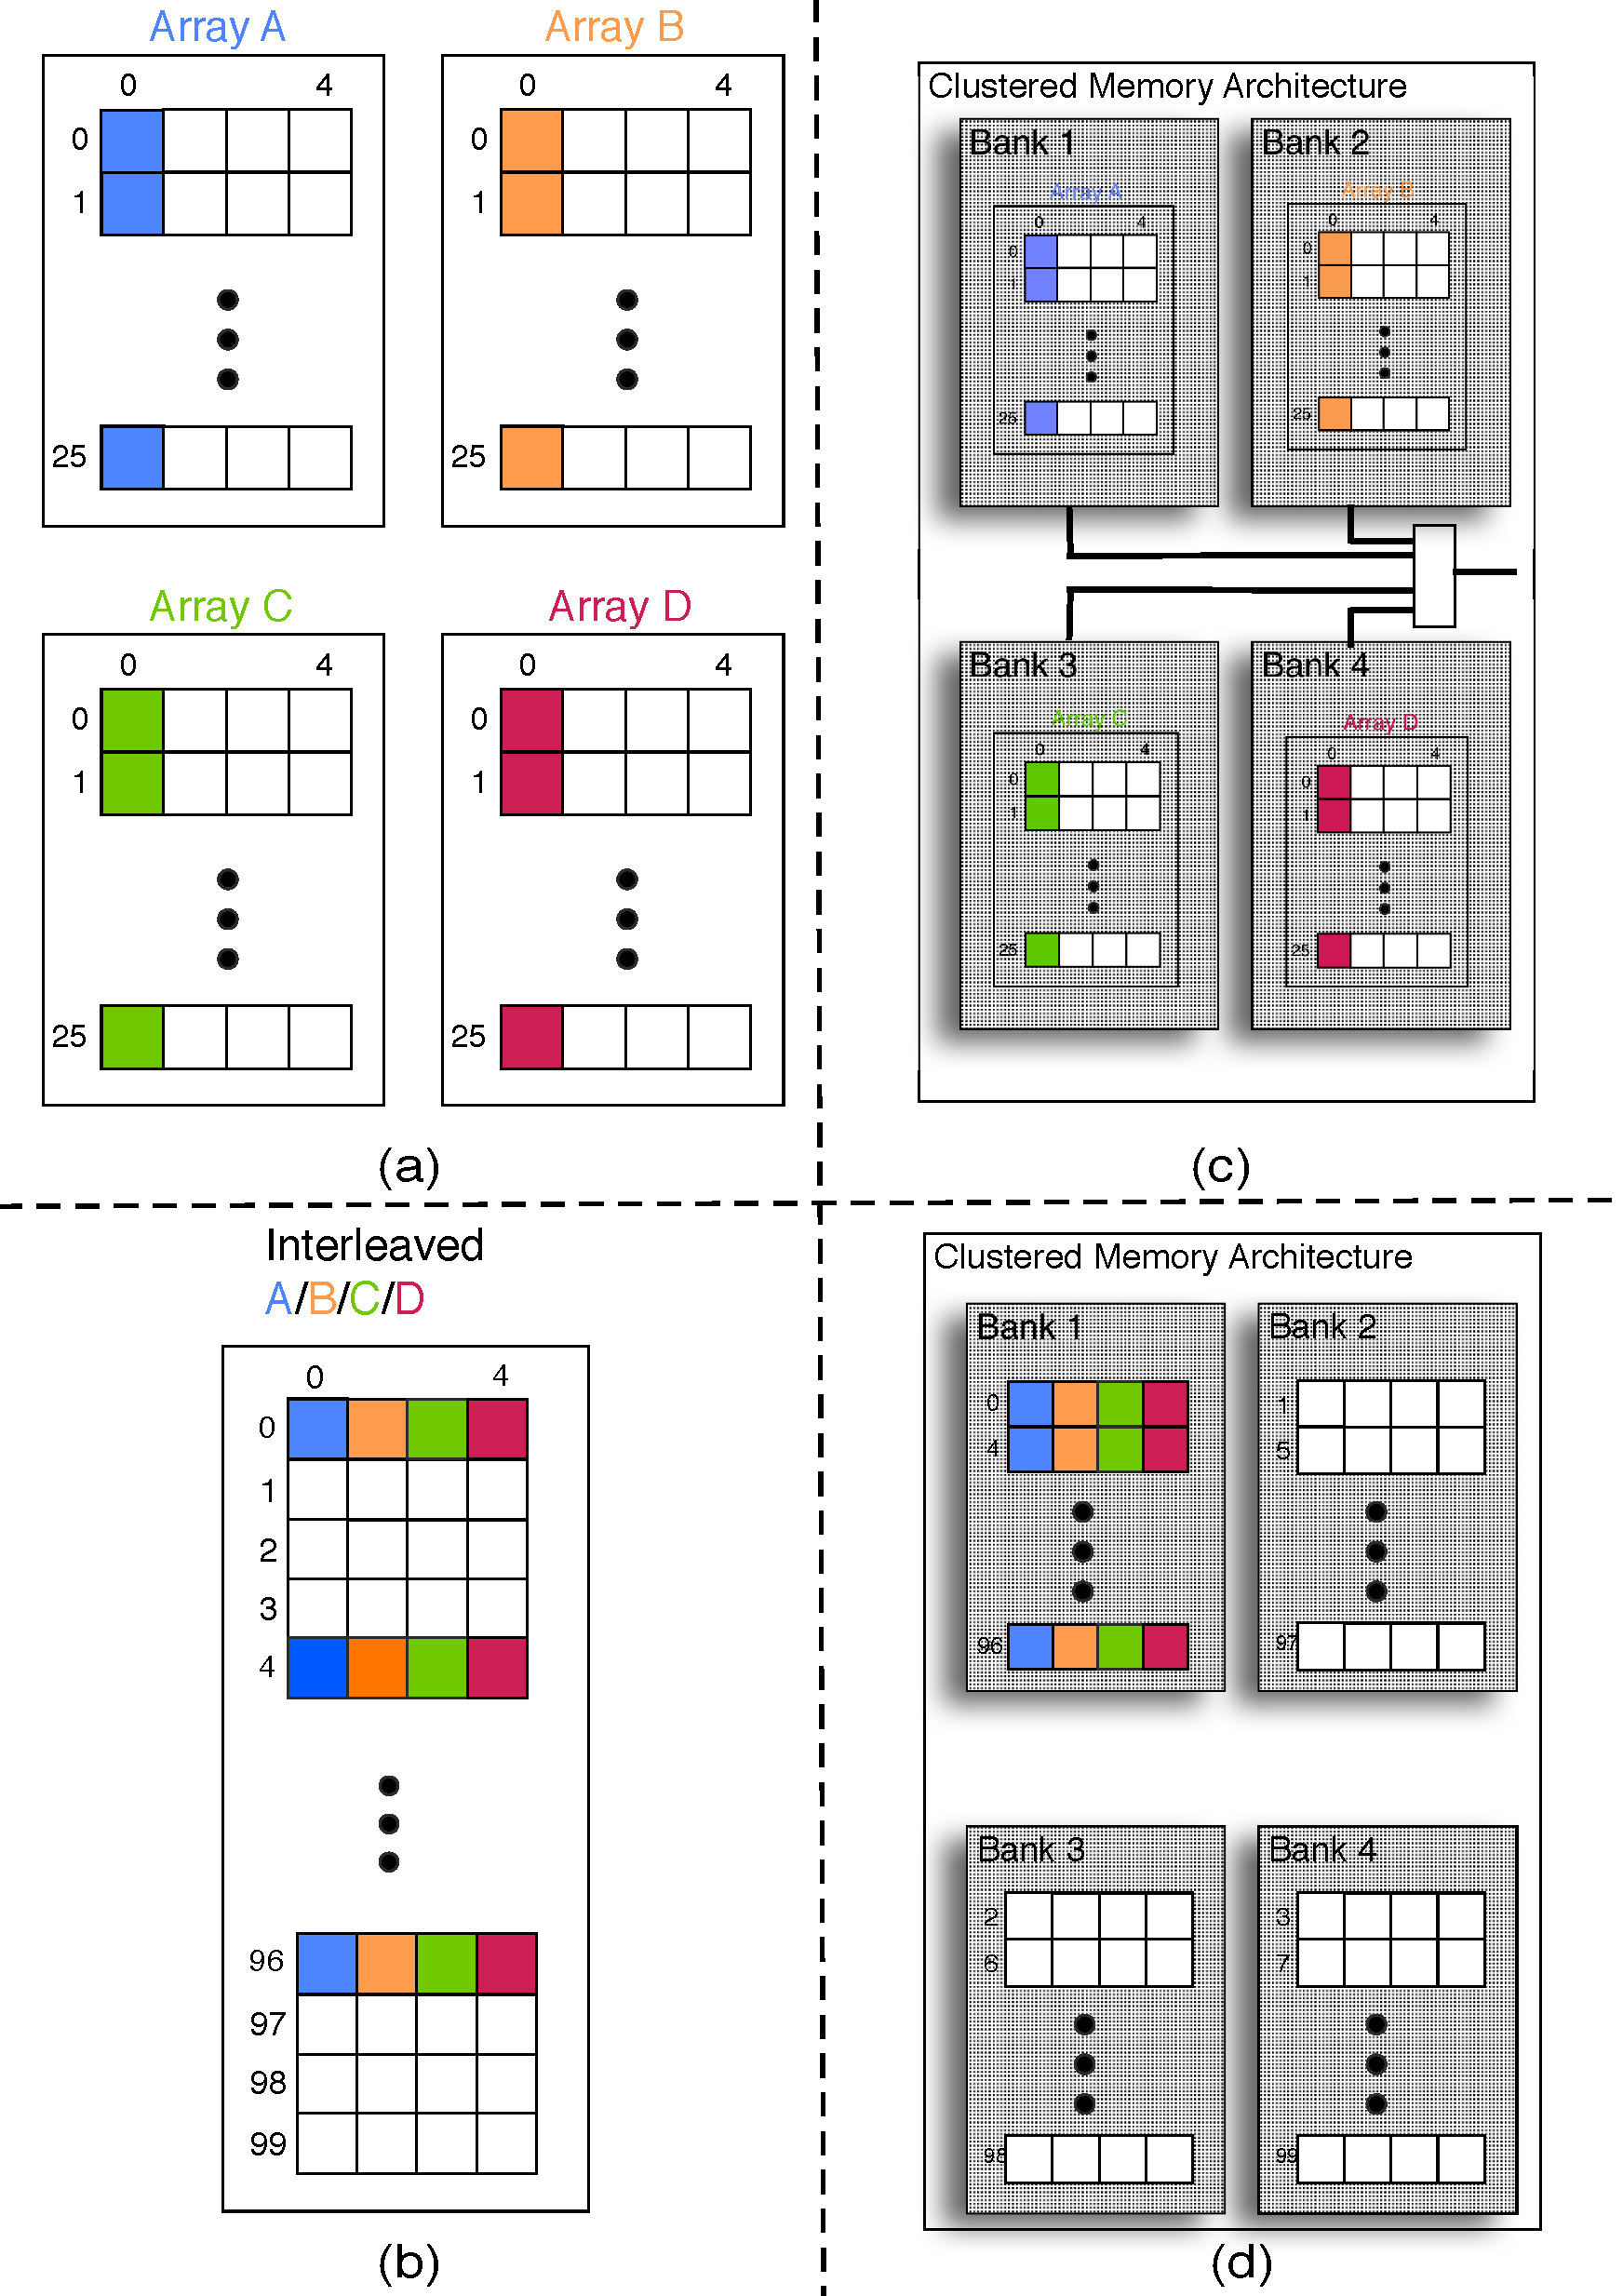
\includegraphics[width = 0.9\linewidth]{D/Images/motivation2.pdf}
	\caption{Motivational Example. Representation of the initial set of data (a) and the interleaved set of data (b). Data-to-memory mapping for the initial (c) and the interleaved data (d) on a clustered scratch-pad memory architecture.}	
	\label{fig:motivation}
\end{figure}

A quick estimation for the difference in the number of memory accesses between the two approaches presented in Fig.~\ref{fig:motivation} can be made.
The target architecture for the current work consists of a reconfigurable clustered memory architecture, a processing element that supports SIMD FUs and a wide bus between them.
The architecture is presented in detail in Sec. \ref{sec:platformD}.
The motivational example uses a system architecture with an SIMD ADD FU that performs operations over 4 array elements at a time and a memory to processor path that has a width of 4 elements. 
Each array element is assumed to have the size of one word.
The register file at the processor level can only store the iteration variable $i$ and 5 elements, which are the variables \textit{result, A, B, C and D}.
Without interleaving of data the number of memory accesses for each loop iteration is 4, because the elements \textit{A(i), B(i), C(i) and D(i)} are stored in different lines and different memory banks or one larger bank.
The overall number of memory accesses is:
	\begin{equation}
		\textit{25 loop iterations $\times$ 4 accesses per iterations = 100 memory accesses}.
	\end{equation}	 
After performing the data interleaving exploration there is only one memory access for each loop iteration, because the elements \textit{A(i), B(i), C(i) and D(i)} are stored in one memory line in the same bank.
The overall number of memory accesses is:
	\begin{equation}
		\textit{25 loop iterations $\times$ 1 accesses per iteration = 25 memory accesses}.
	\end{equation}	 	

A quick estimation for the difference in the energy consumption between the approaches presented in Fig.~\ref{fig:motivation} can be calculated using a simple energy model for the memory banks.
We assume that the energy cost of accessing a memory bank the size of one array is 1E, while the average leakage energy in the time needed for the execution of one loop iteration is 0.3E. 
The corresponding access and leakage numbers for a four times larger memory that can fit all the data together is  3E and 1.2E, respectively. 
The numbers reflects the fact that as a first order approximation access energy increases sub-linearly with increased memory size, while leakage increases linearly with memory size. 
The energy consumption for a large memory with non-interleaved data is:
	\begin{equation}
		\textit{100 $\times$ 3E + 100$\times$ 1.2E = 420E}.
	\end{equation}	
In this case there is a performance loss and an increased leakage energy, because all the accesses has to be done sequentially on the same memory.	
The energy consumption for a four bank memory architecture with non-interleaved data is:
	\begin{equation}
		\textit{100 $\times$ 1E + 4$\times$ 100$\times$ 0.3E = 220E}.
	\end{equation}	
The energy consumption for a large memory with interleaved data is:
	\begin{equation}
		\textit{25 $\times$ 3E + 25$\times$ 1.2E = 105E}.
	\end{equation}	
Finally, the energy consumption for a four bank memory architecture with interleaved data is:
	\begin{equation}
		\textit{25 $\times$ 1E + 1$\times$ 25$\times$ 0.3E = 32.5E}.
	\end{equation}			
It should be noted that the leakage energy in the last case is considered only for the one bank that is always accesses.
The memory banks that store redundant data are assumed switched to retention mode to minimize leakage.
The simple estimations presented in equations (1)-(6) shows that a pure interleaving optimization results in a 75\% reduction in the number of accesses.
A memory optimization based on an energy efficient four bank clustered memory architecture can also give an important energy reduction.
The energy gains are even greater when interleaved data are mapped to an efficient memory architecture.
The observations for this simple example motivates the further exploration of the data interleaving and the data-to-memory mapping for applications with irregularities in their accesses. 
%The performance is also higher as there are 75\% less memory accesses.
%The energy consumption due to memory leakage is also lower, as the access time for the memory and the execution time of the algorithm are shorter.

\section{Related work}
\label{sec:relatedD}

Many studies have been published in the area of data layout transformations and memory management. 
This work differentiates by presenting an integrated approach that combines the two areas. 
The combination is performed in a systematic way and the final result is better than the sum of the two individual optimizations.
The data transformations on the application level are studied in combination with the data-to-memory mapping on the hardware level.
An overview of the related work on those two areas is presented.

Data layout optimizations aim to arrange data in memory with the objective of improving system performance and energy through means such as reduced memory access count or reduced cache misses. 
Several generic data layout techniques have been explored by researchers at various levels in the memory hierarchy. 
In \cite{4},  cache partitioning, a layout technique for arrays, maps each array to different cache partitions to reduce conflicts. 
In \cite{5} authors address the problem for cache miss reduction by evaluating the tiling size for arrays and merging the arrays appropriately for each loop nest. 
Memory Hierarchy Layer Assignment (MHLA), an optimization methodology for data memory hierarchy presented in \cite{6}, determines for each data set an appropriate layer in the hierarchy and type of memory (single/dual port) taking data re-use into account. 
The strategy in \cite{7} partitions the variables to scratch-pad memory and DRAM to minimize interference between variables. 
 The cache-oriented techniques proposed earlier by researchers in \cite{8} do not find a straightforward application in our context, where the target system hardware consists of a scratch-pad memory and a SIMD functional unit.
 The current work explores the assignment of data to the memory and the effect of different interleaving decisions on the overall energy consumption.

Several techniques for designing energy efficient memory architectures for embedded systems are presented in \cite{Mac02}. 
The current work differentiates by employing a platform that is reconfigurable at run-time. 
In \cite{Pgk01} a large number of data and memory optimisation techniques, that could be dependent or independent of a target platform, are discussed. 
Again, reconfigurable platforms are not considered. 
The authors in \cite{Ben00b} present a methodology to generate a static application-specific memory hierarchy. 
Later, they extend their work in \cite{Ben00c} to a reconfigurable platform with multiple memory banks. 

The authors in \cite{abraham1999automatic}, \cite{jacob1996analytical} and \cite{li1999hardware} present methodologies for designing memory hierarchies.
Design methods with main focus on the traffic and latencies in the memory architecture are presented in \cite{chen1999loop}, \cite{grun2000mist}, \cite{jantsch1994hardware} and \cite{passes1995multi}.
Improving memory energy efficiency based on a study of access patterns is discussed in \cite{kandemir2001improving}.
Application specific memory design is a research topic in \cite{schmit1997synthesis}, while memory design for multimedia applications is presented in \cite{oshima1997high}.
The current work differentiates by presenting both a reconfigurable platform and the necessary data interleaving to better exploit the platform.

The current work combines and expands in a non-trivial way, the interleaving exploration presented in \cite{sharma2013data} and the data to memory mapping methodology presented in \cite{filippopoulos2013exploration}. 
In \cite{sharma2013data} a memory dominant application is chosen, which normally suffers from data memory organization bottlenecks while implemented on conventional architectures. 
A data interleaving approach is employed in order to improve memory energy by reducing memory accesses.
Significant reduction in data memory energy consumption can be achieved if array data are interleaved, with no performance overhead.
In \cite{filippopoulos2013exploration} a memory-aware system scenario methodology is presented.
The variations in memory needs during the lifetime of an application are studied in order to optimize energy usage.
Different system scenarios capture the application's different resource requirements that change dynamically at run-time.
Many possible memory platform configurations and data-to-memory assignments are studied as system scenario parameters, which lead to a large exploration space.

\section{Target Architecture and Energy Models}
\label{sec:platformD}

Selection of target platform is an important aspect of the exploration.
The motivational example in the previous section shows that the available choices on the memory models have a great impact on the overall energy consumption.
 The key feature needed in the platform architecture is the ability to efficiently support different memory sizes that are suitable for different data structures.
A generic architecture is presented in Fig.\ref{fig:arch}.
The scratch-pad memory consists of up to four memory banks. 
For more complex architectures the interconnection cost should be considered and analyzed separately for accurate results. 
Although power gating can be applied to the bus when only a part of a longer bus is needed, an accurate model of the memory wrapper and interconnection must developed, which is beyond the scope of the current work.
The SIMD vector FU is assumed to perform instructions on multiple data.

The methodology explores different interleaving and data to memory mapping options for the reconfigurable architecture.
The optimal sizes are found based on the sizes of the data after the interleaving exploration.
The memory banks can operate independently and have different sizes.
The explored data lengths for the vector FU and the connections are 4, 8 and 16 elements.
The exploration is based on the available system models and results in the final system architecture.
Thus, the accuracy of the models influence the decisions taken during the design phase.

\begin{figure}
\centering
	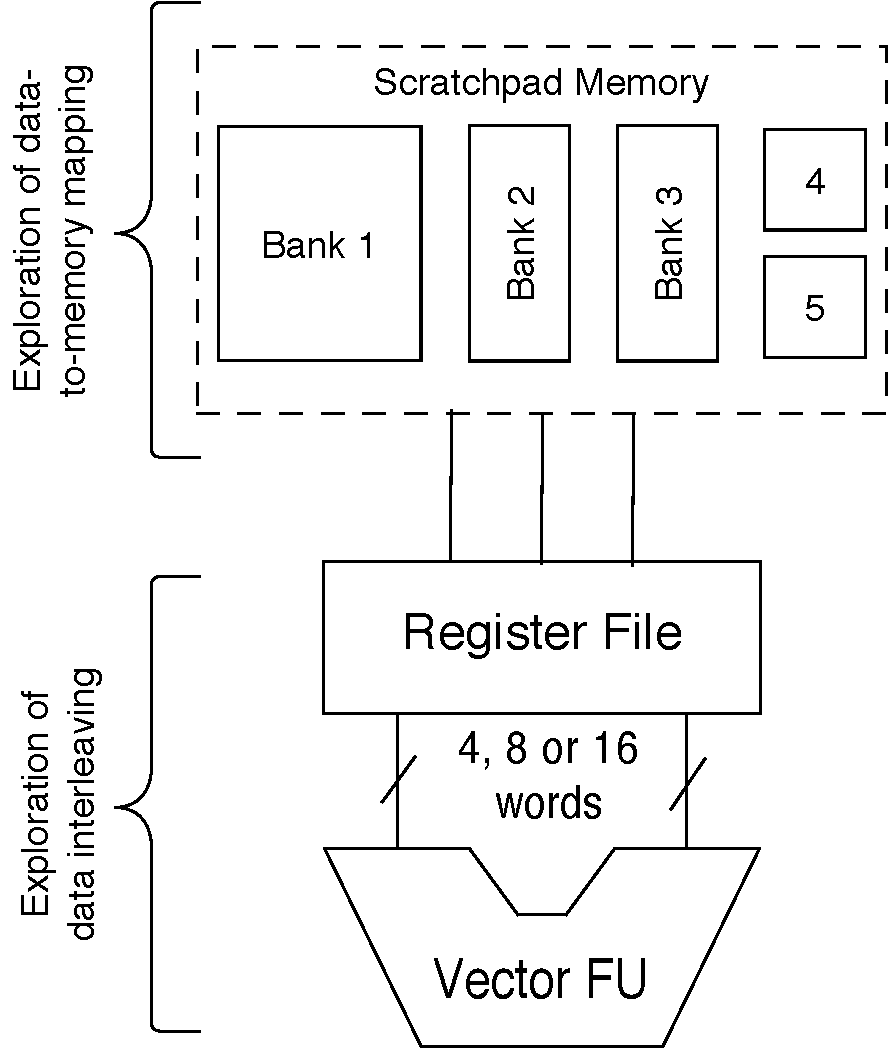
\includegraphics[scale = 0.5]{D/Images/Architecture.pdf} 
	\caption{Exploration options and system knobs depending on a general platform architecture}
	\label{fig:arch}
\end{figure}

\subsection{Memory Models}

The dynamic memory organization is constructed using commercially available SRAM memory models (MM).
For those models delay and energy numbers are derived from a commercial memory compiler.
In addition, experimental standard cell-based memories (SCMEM) \cite{Mei11}  are  considered for smaller memories due to their energy and area efficiency for reasonably small storage capacities, as argued in \cite{Mei10}. 
The standard cell-based memories are synthesized using Cadence RTL compiler for TSMC 40nm standard library. 
Afterwards, power simulations on the synthesized design are carried out using Synopsys PrimeTime, in order to obtain energy numbers.
Both MMs and SCMEMs can operate under a wide range of supply voltages, thus support different operating modes that provide an important exploration space.
\begin{itemize}
\item Active mode: The normal operation mode, in which the memory can be accessed at the maximum supported speed. The supply voltage is 1.1V. 
The dynamic and leakage power are higher compared to the other modes.
Only in active mode the data are accessible without time penalties, in contrast to light and deep sleep modes.
In this work all the memory accesses are performed in active mode. 
\item Light sleep mode: The supply voltage in this mode is lower than active with values around 0.7V. 
The access time of the memory is significantly higher than the access time in active mode. 
Switching to active mode can be performed with a negligible energy penalty and a small time penalty of a few clock cycles (less than 10). 
Data is retained.  
\item Deep sleep mode: The supply voltage is set to the lowest possible value that can be used without loss of data. 
This voltage threshold is expected to be lower for SCMEMs than MM models and can be as low as 0.3V. 
The number of clock cycles needed for switching to active mode is higher compared to sleep mode, typically in the range of 20 to 50 clock cycles depending on the clock speed. 
Consequently, the speed of the PE and the real-time constraints of the applications have to be taken into consideration when choosing light or deep sleep mode at a specific time.  
\item Shut down mode: Power-gating techniques are used to achieve near zero leakage power. 
Stored data is lost. 
The switch to active mode requires substantially more energy and time. 
However, switching unused memories to this mode, providing that their data are not needed in the future, results in substantial energy savings.
\end{itemize}  

The necessary energy and power information is available for the memory models. Relative values for a subset of them is presented in Table \ref{tab:models}. 
It is clearly shown that the choice of memory units has an important impact on the energy consumption.

\begin{table}
\caption{Relative dynamic energy for a range of memories with varying capacity and type}
\label{tab:models}{
	\begin{tabular}{|c|c|c|c|c|c|}
		\hline
		\multirow{2}{*}{\textbf{Type}} & \textbf{Lines x} & \multicolumn{2}{c|}{\textbf{Dynamic Energy [J]}} & \multicolumn{2}{c|}{Switching to Active from} \\ \cline{3-4}
		& \textbf{wordlength} & Read & Write  & Deep[uJ] & Light[uJ]\\ 
		\hline 
		MM & 32 x 8 &  $ 4.18 \times 10^{-8} $ &  $ 3.24 \times 10^{-8} $ & 0.223 &  0.031 \\ 
		\hline
		MM & 32 x 16 & $  6.79 \times 10^{-8} $ &  $ 5.89 \times 10^{-8} $ & 0.223 &  0.031\\ 
		\hline
		MM & 32 x 128 & $  4.33 \times 10^{-7} $ &  $ 4.31 \times 10^{-7} $ & 1.42 & 0.168\\ 
		\hline
		MM & 256 x 128 & $  4.48 \times 10^{-7} $ &  $ 4.60 \times 10^{-7} $ & 1.70 &  0.171\\ 
		\hline
		MM & 1024 x 128 & $  5.11 \times 10^{-7} $ &  $ 5.75 \times 10^{-7} $ & 2.81 & 0.179\\ 
		\hline
		MM & 4096 x 128 & $  9.60 \times 10^{-7} $ &  $ 4.57 \times 10^{-7} $ & 9.01 & 0.457\\ 
		\hline
		SCMEM & 128 x 128 & $  2.5 \times 10^{-7} $ &  $ 0.8 \times 10^{-8} $ & 1.51 &  0.045\\ 
		\hline
		SCMEM & 1024 x 8 & $  1.7 \times 10^{-8} $ &  $ 0.6 \times 10^{-8} $ & 0.325 &  0.021\\ 
		\hline
	\end{tabular}}	
\end{table}

\subsection{Functional Unit Models}

The processing of the interleaved data is performed in the part of the architecture consisting of the SIMD FU and the central vector register file, as shown in Fig.\ref{fig:arch}.
For efficient utilization of the vector FU, the register file has a wide interface (256 bit wide) with the scratchpad memory and allows testing for word length of 4, 8 and 16 elements, assuming that each array element is 16 bit wide.  
This processor belongs to the class of coarse-grain reconfigurable array (CGRA) processors and is described in more detail in \cite{lee2003compilation}.
The HDL model of the processor is synthesized using Cadence RTL compiler \cite{cadencecompiler} and the energy numbers are extracted using Synopsys Primepower \cite{kai2003synopsys}.

For efficient utilization of the vector FU, the register file has a wide interface with the clustered scratch-pad memory. 
Since the target architecture is a configurable processor that can be customized in various ways, the standard evaluation and execution mechanism is to run the programs on a processor simulator. 
An XML based language is used to describe the architecture, and a cycle-accurate simulator of the processor is used to simulate the generated code on the architecture. 
The energy consumption information for different types of instructions and different widths is available for the FU models.
The width of the FU corresponds to the number of pairs of array elements on which the specific instruction is performed.
Relative values for a subset of them is presented in Table \ref{tab:models2}. 
It is clearly shown that the wider FUs have a significantly higher energy consumption compared to FUs that operate on only two element.
Thus, it is important to achieve high utilization of wider FUs to achieve both performance and energy gains.

\begin{table}
\caption{Relative dynamic energy for different FU models}
\label{tab:models2}{
	\begin{tabular}{|c|c|c|}
		\hline
		\textbf{Type of FU instruction} & \textbf{Width} & \textbf{Dynamic Energy [J]} \\ 
		\hline 
		ADD  & 1 & 5.70E-08 \\ 
		\hline
		ADD  & 4 & 2.28E-07 \\ 
		\hline
		MULT  & 1 & 2.48E-07 \\ 
		\hline
	 	MULT complex  & 1 & 5.33E-07 \\ 
		\hline
		MULT  & 4 & 1.03E-06 \\ 
		\hline
		MULT complex  & 4 & 1.95E-06 \\ 
		\hline
		\end{tabular}}	
\end{table}

\section{System Design Exploration Work-flow}
\label{sec:methodologyD}

\begin{figure}
\centering
	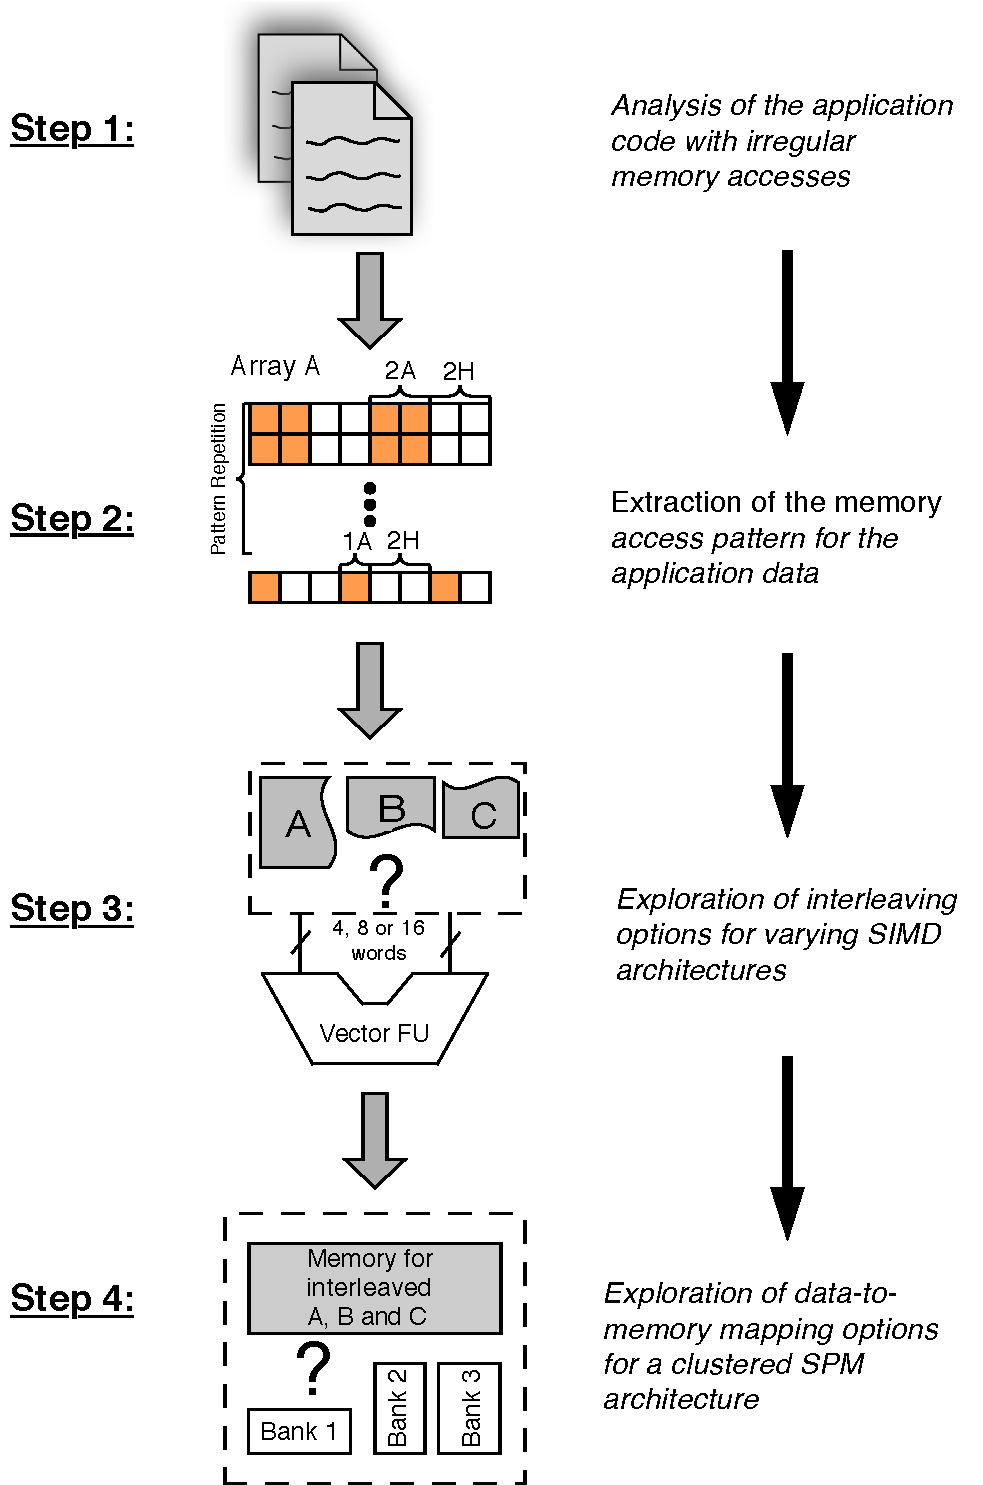
\includegraphics[scale = 0.6]{D/Images/workflow2.pdf} 
	\caption{Methodology steps}
	\label{fig:workflow}
\end{figure}

As motivated in the previous sections a systematic exploration of the interleaving options and the data-to-memory mapping possibilities is necessary.
The input to the work-flow is the application code and the output of the exploration is an efficient solution for the interleaving of the data and a mapping to a reconfigurable system architecture based on the available models presented in Sec.\ref{sec:platformD}.
The exploration space consists of the potential combinations between the different arrays and the different scratch-pad memory architectures, which combine memories of different types and sizes.

The overall work-flow is presented in Fig.\ref{fig:workflow}. 
The first step of the methodology is the analysis of the application code. 
The methodology is applicable to any application.
However the applications that can benefit more from the proposed methodology are the ones with irregular access patterns.
The second step is the extraction of the access pattern for each data structure present on the application code.
The third step is the interleaving exploration, which explores all the different options for the re-arrangement of the data.
The aim of this step is the construction of compact sets of data by using defined operations between the available access patterns.
The goal is to better utilize the different width of the vector FUs. 
The result of the interleaving is a set of data with a reduced number of holes.
The forth step is the mapping of the interleaved data set to the clustered memory architecture.

Some significant changes are needed in order to combine the different techniques in a functional work-flow.
The interleaving and the data-to-memory mapping exploration steps have to be modified and a simple concatenation is not sufficient.
The results of the interleaving exploration are given as constraints to the mapping exploration.
The constraints stir the exploration in a potentially different solution compared to the result of the data-to-memory mapping exploration without the interleaving constraints.
The interleaving exploration finds solutions for the different bus widths and then all the different solutions are propagated to the mapping exploration.
The mapping exploration takes all the interleaving constraints into consideration.
Thus, the data-to-memory mapping solutions using the constraints are in general different from the solutions provided in a conventional approach.
The propagation of the constraints is explained in more detail later. 

\subsection{Formal Model Representation of Access Patterns }

A representation model for the memory access patterns is employed in order to formally present each step of the methodology.
The model presented in \cite{Ang13} is a generic model suitable for irregular iteration spaces on arrays.
The irregularities are created by the application code access statements in a conditional loop structure.

When an array element is accessed during the code execution, it is represented with an A(Access).
Otherwise, there is a hole in the access pattern represented with an H(Hole) as shown in Fig.\ref{fig:pattern}.
The sequence of accesses and holes is usually repeated periodically, because normally the loop conditions are not totally random.
Thus we can define the frequency of each access pattern.
The analysis of the application code results in the access patterns and their corresponding frequencies, which is the necessary input for the next step in the work-flow.

\begin{figure}
\centering
	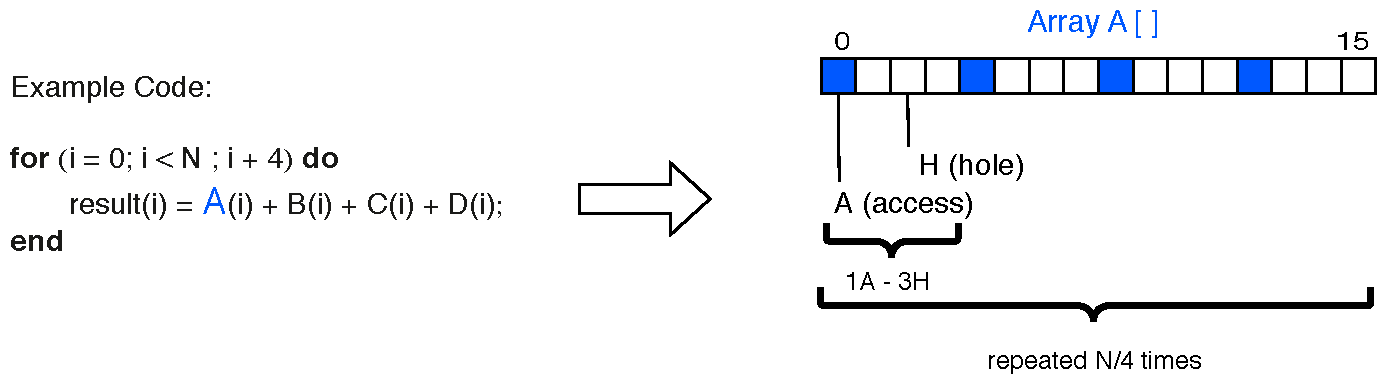
\includegraphics[scale = 0.6]{D/Images/AHpattern.pdf} 
	\caption{Extraction of access pattern from application code}
	\label{fig:pattern}
\end{figure}

%\textit{Discussion about polyhedral and enumerative approaches}
%\textit{Analysis of A-H model based on Angeliki}
%\textit{Definition of algebra functions between access patterns}

\subsection{Data Interleaving Exploration}
Interleaving is a data layout transformation for combining the storage of multiple arrays, so that blocks of data from different arrays are stored contiguously, in order to achieve spatial locality in memory accesses.
By interleaving we are able to group the data to be accessed and thus reduce the number of memory accesses for accessing them.
The basic principles of the performed interleaving exploration are presented in \cite{sharma2013data}.

The employed model of access pattern representation is accompanied with a suitable algebra presented in \cite{kritikakou2013phd}.
The operations defined help the designer explore different interleaving options.
The goal of the process is to rearrange the data in an efficient way to increase the number of sequential accesses.
A simple example is presented in Fig.\ref{fig:algebra}.
Arrays $A$ and $B$ are interleaved by interchangeably storing an element of each array in the new array. 
The access patterns of arrays $A$ and $B$ are combined in a new access pattern, which has two accessed elements placed consecutively.
The use of access patterns and the theory for calculating the access patterns of different combinations enables an extensive exploration of the possible data interleaving options.

The impact of the data interleaving exploration on the number of memory accesses is significant.
When the accesses are irregular and the data are organized in index order, each memory access results in a small amount of useful data due to the presence of holes.
In contrast the re-organization of the data provides a sequence of useful data without many holes between them.
Thus, a single access to the memory results in a higher number of useful elements.
The overall number of memory accesses is reduced, as each access has a higher utilization.

This idea is illustrated in Fig.\ref{fig:algebra}.
The number of memory accesses for each case can be calculated by assuming that each memory access loads four array elements, i.e. the word length for the memory and bus architecture is four elements.
Each time an element from the array $A$ or $B$ is needed, the memory access returns four elements, from which one is the useful and the other three are not used by the running code.
In the case of the interleaved array, each memory access returns four elements, from which two are useful and two redundant.
Thus, the overall number of memory access in the second case is reduced by half compared to the first case.

\begin{figure}
\centering
	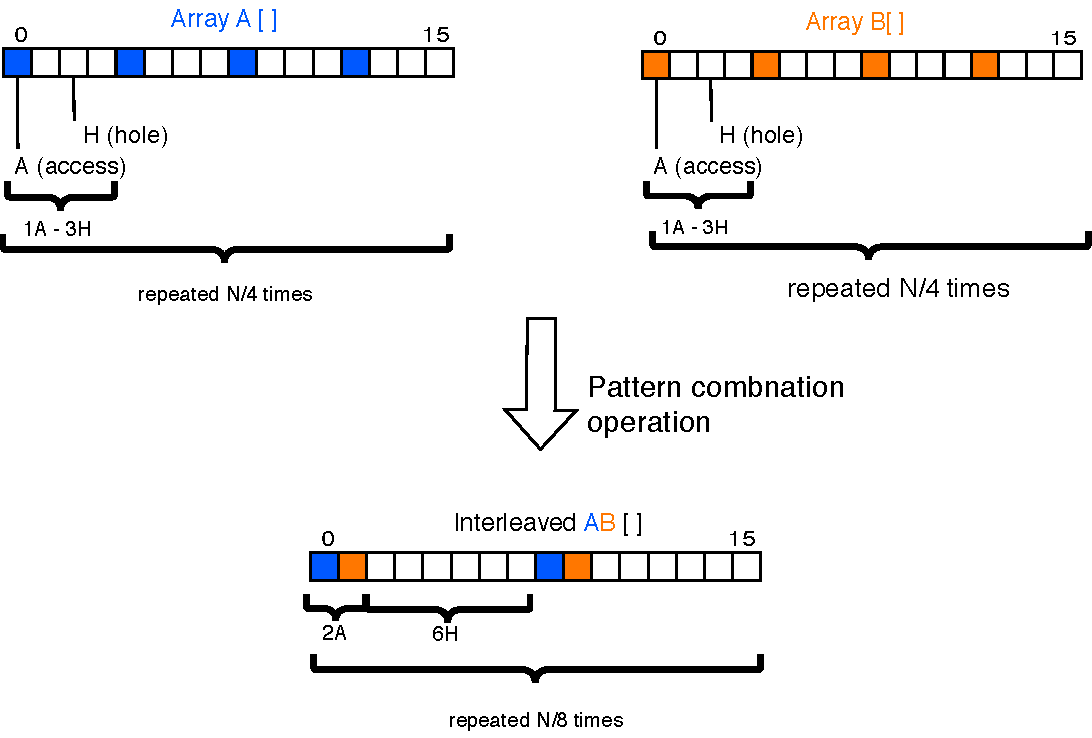
\includegraphics[scale = 0.6]{D/Images/Algebra.pdf} 
	\caption{Example of combination between two arrays and their access patterns}
	\label{fig:algebra}
\end{figure}
%\textit{Algorithm for exploring data interleaving}

\subsection{Data-to-Memory Mapping Exploration}

Given the input from the previous step, we explore the mapping of the interleaved data to the memory architecture.
A clustered memory organisation with up to five memory banks of varying sizes is explored. 
The limitation in the number of memory banks is necessary in order to keep the interconnection cost between the processing element (PE) and the memories constant through exploration of different architectures. 
The decision to use memory banks with varying sizes on the clustered memory organization increases the reconfiguration options and consequently the potential energy gains. 
In general, smaller memories are more energy efficient compared to larger memories banks. 
However, in some cases large memory banks are needed in order to fit the application data without the need for too many small memories causing complex interconnects. 
The goal is to use the most energy efficient banks to store the interleaved data.

The exploration space consists of different sizes and types of memory banks.
The goal is to select the optimal set of memory banks and to make  the optimal decision regarding the mapping of the data to the different memory banks.
The parts of the interleaved data that consist mostly of useful elements are mapped into memory banks with low energy per access but at the same time with the necessary access time.
The parts of the interleaved data that consist of access holes and rarely accessed elements are optimally mapped into memory banks with energy efficient retention states.
In both cases the size of  the memory banks should be adequate to fit the stored data but at the same time as small as possible to avoid area and energy penalties.

\subsection{One way constraint propagation}

The interleaving decisions influence the data-to-memory mapping decisions and vice versa.
For example, the decision to interleave two arrays \textit{A and B} have an impact on the freedom of mapping the interleaved array $A\vert B$ on the memory banks, because of the difference in size and structure.
The data-to-memory mapping decisions affect the interleaving decisions in a similar way.
Assuming that the mapping is performed first using the initial data the following interleaving options are reduced.
For example, the decision to map two arrays on different memory banks removes the option to interleave them later.
Optimizing both the interleaving and the memory mapping at the same time results in a large and inefficient loop of constrain propagations between the two exploration phases.
 
We choose to perform the interleaving exploration step first and then propagate the most efficient interleaving options to the data-to-memory mapping step.
The code and data transformations should be performed earlier to avoid omitting possible solutions as justified in \cite{dtse}.
Thus, the interleaving decisions are propagated as constraints on the mapping exploration phase. 
The constrains consist of the arrays that are interleaved, the new access pattern and the width of SIMD architecture for which the specific interleaving solution is optimal.
The mapping step is performed based on these constrains.

\section{Applications}
\label{sec:applicationsD}

The applications that benefit most from the proposed methodology are characterized by having irregular access patterns with holes.
Applications with irregular accesses can be found on several application domains.
The current study includes representative candidates from three different domains, namely the multimedia, the wireless and the equation solver domains.
Suitable applications can also be found on other areas.
An overview of the tested benchmark applications is presented below:

\begin{enumerate}
\item Motivational example is the very simple example presented in Sec.~\ref{sec:motivationalD}. 
It uses four arrays that all have the same irregular access pattern, namely 1A-3H.
One element from each array is used to calculate an intermediate result on every loop iteration.
The interleaving is easy because the four arrays have the same pattern.
Further interleaving within the array can result in even longer sequences of useful elements.
The access pattern is repeated for every four elements (1A-3H), so the scaling for the different word lengths (4, 8 and 16) is expected to be good. 
\item Successive Over Relaxation (SOR) is a method for evaluating partial differential equations or solving a linear system of equations.
The SOR benchmark has a more irregular access pattern.
The interleaving exploration provides sequences of three or six sequential useful elements.
Thus, the utilization on the SIMD architecture is expected to be lower.
This application is an representative example from the equation solver domain.
\item FFT benchmark has an irregular pattern during the access of the pilot matrices. 
The interleaving exploration for FFT is presented in \cite{sharma2013data}.
The number of matrices is higher and more interleaving options are present.
However, the interleaving cannot provide an acceptable solution for 16 sequential useful elements.
This application is an representative example from the wireless domain, because FFT is widely used on wireless applications.
\item Motion estimation benchmark is a dynamic algorithm that results in different access patterns based on the identification of the moving objects. 
The static parts are not accessed resulting in holes in the accesses and the interleaving aims to minimize those parts.
The interleaving exploration provides alternatives for all the  tested word lengths. 
This application is an representative example from the multimedia domain.
\end{enumerate}

\section{Results}
\label{sec:resultsD}

%\begin{table}%
%\tbl{Normalized energy consumption\label{tab:results}}{
%\begin{tabular}{c c}
%\includegraphics[width=0.45\linewidth]{Images/Example.pdf} & \includegraphics[width=0.45\linewidth]{Images/sor.pdf} \\
%\includegraphics[width=0.45\linewidth]{Images/fft.pdf} & 
%\includegraphics[width=0.45\linewidth]{Images/mest.pdf} 
%\end{tabular}}
%\end{table}

The design exploration is applied to the chosen application benchmarks and energy numbers are derived based on the described target platform.
The energy numbers are calculated both for the memory and the SIMD architecture presented in Sec.\ref{sec:platformD}.
Four approaches are explored and the corresponding energy consumption for each of them is calculated.

\begin{itemize}
\item \textit{No optimization.} 
In this case there is no interleaving exploration and the memory architecture consists of one large memory bank. All the data are mapped on the memory bank without any optimization. 
\item \textit{Memory Size Optimization.} 
In this case there is no interleaving exploration and the memory architecture consists of five memory banks.
The optimal size for the memory banks and the optimal mapping of the non-interleaved data on them is explored. 
The number of memory accesses is the same as in the previous approach.
However, the data is mapped on an efficient clustered memory architecture.
\item \textit{Interleaving optimization.} 
In this case the  interleaving exploration step is performed and the memory architecture consists of one large memory bank.
The optimal interleaving decision is found and applied to the data, so the locality of useful data is increased.
However, all the data are mapped on one large memory bank.
The number of accesses is significantly reduced by the interleaving step, but the energy per access is kept high due to lack of data mapping to an efficient clustered architecture.
\item \textit{Integrated co-exploration.} 
In this case the co-exploration of both the interleaving and the data-to-memory mapping optimizations is performed.
Both he number of memory accesses and the energy per access are reduced.
\end{itemize}

\subsection{Motivational Example}

\begin{figure}
\centering
	\includegraphics[scale = 0.5]{D/Images/Example.pdf} 
	\caption{Motivational Example}
	\label{fig:example}
\end{figure}

The normalized energy consumption for the motivational example is presented in Fig.\ref{fig:example}.
The four different approaches are normalized using the monolithic approach without any optimization.
Energy results for this benchmark are presented for a bus width of 4, 8 and 16 elements, which means that every memory access loads/stores 4,8 or 16 elements. 
The interleaving exploration proposes three different solutions for an SIMD architecture width of 4, 8 and 16 elements respectively.
The data access patterns of the three interleaving decisions are propagated as a set of constrains to the mapping step.
The mapping step explores all the different data-to-memory mapping options and proposes the most energy efficient memory organization for each of the three interleaved data solutions.

The application code is perfectly suited for interleaving as discussed in Sec.\ref{sec:motivationalD}.
Thus the interleaving exploration has a greater impact than the memory size optimization.
However, the integrated approach optimizes the energy consumption even further.
The application is suitable for higher bus widths and there are important gains while moving from 4 to 8 and 16.
The increase in the architecture width result in significant gains even without any optimization.
The gains are approximately 50 and 70\% for a width of 8 and 16 compared to a width of 4.
This is explained by the fact that the accessed array elements are close enough even without data transformations and the existence of holes in the access pattern. 
By fetching 8 and 16 elements from the memory, the number of useful elements is two and four times more.
Studying the motivational example in Fig.\ref{fig:example}(a) for a width of 16, each access results in 4 lines with one colored element each.

The interleaving optimization results in greater improvements compared to the memory optimization.
This is explained by the nature of the application that offers good interleaving options for larger words, i.e. higher values of bus width.
The memory optimization is around 20\% lower than the monolithic approach for any width.
The interleaving optimization results in more than 70\% lower energy for a width of 4 and more than 80\% for a width of 8 and 16.
The interleaving of the arrays provides perfectly compact sets of data as shown in Fig.\ref{fig:example} and the interleaving cannot improve more for higher values of width.
The great impact of the combined approach is better illustrated for a width of 16. 
In this case the two optimizations alone report an energy gain around 20\% and 35\% compared to the non optimized case for width of 16.
The combined approach results in an energy gain of 84\% on the same case.

\subsection{SOR Benchmark}

\begin{algorithm}
\caption{Code snippet from the SOR benchmark}
\label{alg:sor}
\begin{algorithmic}[1]
\STATE $...$
\STATE $N \gets 100$
\FOR {$j = 0 \to N$}
	\STATE $resid \gets c(i)(j) \times u(i)(j-1) + d(i)(j) \times u(i)(j) + e(i)(j) \times u(i)(j+1) $ 	
	\STATE $j \gets j+2$
\ENDFOR	
\STATE $...$
 \end{algorithmic}
\end{algorithm}

\begin{figure}
\centering
	\includegraphics[scale = 0.5]{D/Images/sor.pdf} 
	\caption{SOR Benchmark}
	\label{fig:sor}
\end{figure}

The normalized energy consumption for the SOR benchmark is presented in Fig.\ref{fig:sor}.
The four different approaches are normalized using the energy consumption of a system without any optimization as the base.
Energy results for this benchmark are presented for a bus width of 3 and 6, although the architecture supports bus widths of the power of 2.
This means that every memory access loads or stores 4 or 8 elements, but only up to 3 or 6 array elements are used in the algorithm.
This limitation is due to the nature of the application code that adds elements from 3 arrays to 3 sequential elements of another array. 
Alg.~\ref{alg:sor} is a code snippet that demonstrates the considered data structures.
The arrays \textit{c, d and e} are potential candidates for the interleaving exploration.
The interleaving exploration on the application code concludes that it is only possible to make sequential sets of 3 and 6 elements by interleaving the arrays \textit{c, d and e}.
The elements that are multiplied with them are already sequential.

 The interleaving exploration has a small impact on the reduction of energy consumption for a bus width of 3 elements.
 This is due to the addition of a redundant element, in order to have a width of four that is supported by the architecture.
The results are even worse for a bus width of 6 elements, because there is a need for two redundant elements to comply with a set width of eight.
The mapping of the initial data to a clustered memory results in a reduction of around 20\%, which is slightly better than the interleaving optimization.
The reason is that the mapping of the initial data demands all the memory banks active and the memory is heavily accessed during the execution of the benchmark.
The integrated approach exploit on a better way the few interleaving options and provides a better mapping of the interleaved data to the memory architecture.
The final gain for a width of three is 47\%, compared to 17\% and 20\% for the interleaving and the memory optimization respectively.

\subsection{FFT Benchmark}

\begin{figure}
\centering
	\includegraphics[scale = 0.5]{D/Images/fft.pdf} 
	\caption{FFT Benchmark}
	\label{fig:fft}
\end{figure}

The normalized energy consumption for the FFT benchmark is presented in Fig.\ref{fig:fft}.
The four different approaches are normalized using the monolithic approach without any optimization.
Energy results for this benchmark are presented for a bus width of 4 and 8 elements, which are the two viable options provided by the interleaving exploration.
Again, the integrated approach results in the lower energy consumption.
The energy gains for a bus width of 8 are significant, because blocks of 8 elements can be constructed by interleaving of application's arrays.

\subsection{Motion Estimation Benchmark}

\begin{figure}
\centering
	\includegraphics[scale = 0.5]{D/Images/mest.pdf} 
	\caption{Motion Estimation Benchmark}
	\label{fig:mest}
\end{figure}

The normalized energy consumption for the motion estimation benchmark is presented in Fig.\ref{fig:mest}.
The four different approaches are normalized using the monolithic approach without any optimization.
Energy results for this benchmark are presented for a bus width of 4, 8 and 16 elements.
The application code provides good possibilities for interleaving and consequently the interleaving exploration has a greater impact than the memory size optimization.
However, the integrated approach optimizes the energy consumption even further.
In this case the energy gains for increasing size of bus width are minimal when only one optimization is applied.
This is explained by the nature of the application, which has large parts of redundant data spread out through the memory.
Thus, the whole memory is active when the mapping is not performed on the compact interleaved data.
The combined approach offers significant energy gains even for the highest bus width. 

\section{Conclusion}
\label{sec:conclusionD}

The scope of this work is to presents a methodology for efficient exploration of data interleaving and data-to-memory mapping options for SIMD (Single Instruction Multiple Data) platform architectures.
Detailed energy models are presented for the studied architecture.
The methodology focuses on reducing the overall energy consumption by reducing the number of memory accesses and the energy per access.
The number of memory accesses is reduced by interleaving the application data to construct compact sets of sequential data.
The energy per memory access is reduced by employing a reconfigurable scratch-pad memory architecture with multiple banks that can operate independently.
A systematic way is presented in order to explore the different options that lead to the interleaving and data-to-memory mapping decisions.
A wide range of applications is studied that allow us to draw conclusions about different kinds of dynamic behavior and their effect on the energy gains achieved using the methodology. 
The improvement in the total system energy consumption after efficient interleaving and mapping of data is between 40\% and 80\% for the studied benchmarks having the type of irregularities in their access scheme that benefit most from the methodology.

% Bibliography
\addcontentsline{toc}{section}{Bibliography}	
\bibliographystyle{plain}
\bibliography{reference}
%\bibliographystyle{ACM-Reference-Format-Journals}
%\bibliography{reference}
